% Software Backend (Python)
% Zuständig: Jones

% wie/wo soll protobuf erklärt/erwähnt werden?

\chapter{Software - Backend}
\label{sec:software_backend}
\initials{JS}
Das Backend ist die Zentrale Rechenstelle, 
welches in mehrere Komponenten aufgeteilt ist.
% generell zum backend

\begin{figure}[H]
    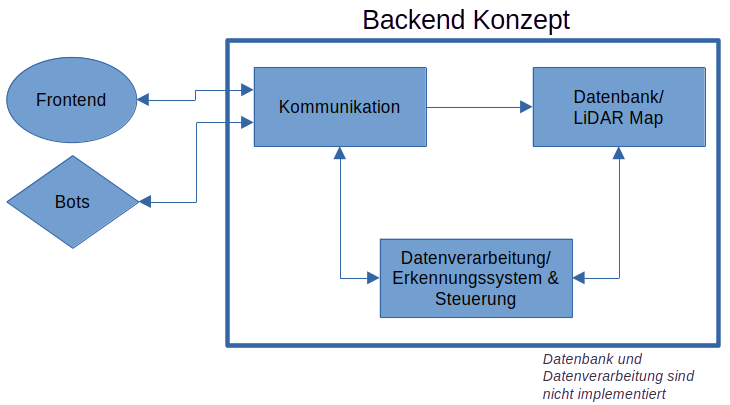
\includegraphics[width=\textwidth, center]{img/backend-konzept.png}
    \caption{Backend Konzept}
    \label{fig:backend_konzept}
\end{figure}
% grafik anpassen

Wodurch es verantwortlich für die Kommunikation und Datenerfassung 
zwischen allen Teilnehmer. 
Dazu gehören die drei Roboter, welche uns die Daten liefern 
wie LiDAR, Beschleunigungssensor etc., 
und das Frontend zu dem die Daten zur Visualisierung und Mitverfolgung gesendet werden
und gegebenenfalls auch Befehle empfingt.
\\
Weiters findet hier die Zentrale Datenverarbeitung und Verwaltung statt, 
dies ist verantwortlich für die Erstellung der LiDAR Map, 
der Ermittlung der Roboter Positionen 
und gegeben falls Berechnung der Messwerte. 
% im falle ineffizient etc
\\
Und Steuerung der Roboter mithilfe eines Erkennungssystems 
welches bestimmte Kennzeichen in den erhaltenen Daten Ausschau hält und 
darauf Kennzeichen für die einzelnen Bots erkennt und verfolgt, 
um entsprechend die Positionen aller Bots relativ zur LiDAR Map ausfindig zu machen.
% 
% Die Zentrale Datenverarbeitung und autonome Steuerung der Roboter sind 
% im zu zeitigen Prototypen stand nicht implementiert.
% % stattdessen weiterleitung und fernsteuerung
% TODO 
\\
Und letztendlich die Datenbank welches die etwaigen Daten speichert 
von der Datenverarbeitung und Erkennungssystems, 
dazu gehört insbesondere die LiDAR map.

Für das Backend wurde Python gewählt, 
welches von seiner Vielzahl von Standardpaketen und 
großen Anzahl an externen Paketen und Frameworks, 
eine effiziente und schnelle Programmierung ermöglicht, 
auch unterstützt durch eine aktive Community.
% 
Für dieses Projekt wurde es gewählt aufgrund seiner Vielseitigkeit, 
speziell in Bezug auf den unterschiedlichen Task die ausgeführt werden müssen, 
hauptsächlich der Kommunikation und Datenverarbeitung 
Felder in die Python üblicherweise verwendet werden.
% 
Darauf müssen auch mehrere Verbindungen offen bleiben und verwaltet werden,
und dies schnell zu realisieren mithilfe von Paketen 
die uns ermöglichen aufs wesentliche zu fokussieren.
% 
Eine schnelle Programmierung und Modifizierung, 
weil das Backend voraussichtlich mit dem zum zeitigen Projektstand wächst, 
ganz wichtig für die Datenverarbeitung und Steuerung 
da diese sich im Laufe des Projekts stark ändern kann,
aufgrund dessen, dass die Methoden und Systeme nicht endgültig feststehen, 
und teilweise noch definiert werden müssen.
% 
Und letzteres auch wegen Erfahrungen mit dem Vorgänger Projekt, 
denn ein wesentlicher Teil davon bestand auf die Kommunikation über Websockets.
% Gelaber über python
% wegen math Funktionen...
% schnelle Modifizierung 
% packet/ Bibliothek Fokussierung auf Einfachheit
\section{Systembeschreibung}
\initials{JS}
% drunter verschoben weil besseres layout?
In disem Abschnitt wird genauer 
über die geplanten einzelnen Komponenten gesprochen 
und deren Funktion.

Zu beachten ist, dass nicht alle geplanten Systeme, die hier Beschrieben sind,
implementiert wurden und manche noch in der Konzeptphase sind.
Für den tatsächlichen Stand siehe Abschnitt \ref{subsec:backend_aktueller_stand}.

\subsection{Datenverwaltung}
\label{subsec:backend_data}
\initials{JS}
% übersicht über die drei komponenten und wie ungefähr der datenfluss aussieht?
TODO
% Datenbank für lidar?
TODO

Dieser Abschnitt bespricht kurz den Datenablauf 
zwischen den Teilnehmer und den internen Komponenten.
% 
Weil die Datenverarbeitung noch nicht realisiert ist 
kann noch nicht viel weiter zur Verwaltung gesprochen werden.

Das Frontend und die Roboter kommunizieren hauptsächlich 
über Websockets mit den Protobufs.

\subsection{Kommunikation}
\label{subsec:Kommunikation}
\initials{JS}
Die drei Roboter sind aktive Teilnehmer in der Kommunikation, 
das heißt es ist zu erwarten, dass die Verbindung konstant aufrechtzuerhalten ist,
bidirektional und dies auch in einem zeitlichen verhalten geschieht. 
Insofern muss weiter sichergestellt werden das ein konstanter Kommunikationsfluss 
ermöglicht bleibt.

Zur Verbindung entschieden wir uns für das Kommunikations-Protokoll Websocket, 
diese ermöglicht eine bidirektionale, 
persistente Verbindung zwischen einem Client und einem Server,
welches im Vergleich zu gewöhnlichen HTTP-Anfragen offen bleibt, 
wodurch Echtzeitkommunikation möglich ist.
% könnte man mehr ausschreiben aber schau ma später

\subsection{Datenverarbeitung}
\initials{JS}
% TODO
Ein Teil des Servers ist die Verarbeitung der erhaltenen Daten, 
die entweder zum Frontend weitergeleitet wird, oder vom Server verarbeitet.
% 
Um große Belastung mit Sensordaten Berechnung auf den Roboter zu vermeiden,
werden einige Arbeiten auch auf den Server entlasten.
Ein weiterer Grund dafür ist, aufgrund dessen das mit Python 
bereits ausgebaute Mathematik Pakete zur Verfügung stehen
und die Sensordaten zu Bearbeiten.
Und auch ausgebautes Daten Analyse und Manipulation Pakete.


\subsection{Erkennungssystem}
\initials{JS}
Geplant war das die erhaltenen Daten über das Datenverarbeitungssystem 
über die Zeit hinaus eine Karte erstellt sozusagen die LiDAR map,
welche in einer Datenbank abgespeichert werden.
% 
Über die Zeit werden Datenpunkte gesammelt, 
die sich mehr nach einem gewissen Muster sammeln 
und ein klareres Bild über die Form eines Raumes geben.
Diese Muster, wie gerade Linien und Ecken werden vom System erkannt
und mit diesen Eigenschaften auch ermittelt, 
wo ungefähr sich der Guide im Raum befindet.
% 
Dies wird mit einem weiteren Erkennungssystem für Tamerlan \& Bambi,
welches zuständig ist die position der zwei zu ermitteln.
Indem die Bots identifizierbare reflektieren Objekte befestigt kriegen,
Beispielweise mehrere Zylinder wodurch sie erkannt werden können.
%
Mit diesen Informationen kann die Steuerung der Roboter folgen.
% füge skizzen hier oder erklär anderen Kapitel?
% Kugel, stab, mehrere stäbe, reflektierendes material

Eine genauere Beschreibung der LiDAR Karte und wie diese aussieht
ist im Frontend Abschnitt \ref{subsec:frontend_lidar_map} 
auf Seite \pageref{subsec:frontend_lidar_map} zu finden.

\subsection{Steuerung der Roboter}
\label{subsec:backend_robot_detection}
\initials{JS}
% TODO
Zurzeit nicht realisiert.
% spätester schritt weil funktionierende Strategie benötigt wird zur Erkennung
% Datenbank/ Datenbearbeitung

Die Aufträge der einzelnen Bots sind in den Entsprechenden Kapitel genauer beschrieben.
% schau was da steht und was speziell hier klargemacht werden muss

Es sind zwei Steuerungen geplannt die manuelle Steuerung 
und die Automatisierte.
% 
Die manuelle Steuerung geschieht über das Frontend 
womit man die Roboter mit hilfe der Visualisierungen 
und oder Video Übertragung steuern kann.
% 
Die Automatisierte Steuerung geschieht mithilfe das Erkennungsystem 
und soll die Bots erlauben die erstellte LiDAR Karte zu navigieren
und erlauben die zwei Blinden Bots Tamerlan \& Bambi den Guide zu folgen.
% verwendung von code vom vorgänger Projekt

\section{Aktueller Stand}
\label{subsec:backend_aktueller_stand}
\initials{JS}
% Womöglich Teile zu Ergebnisse verschieben?
Zum Zeitpunkt dieser Diplomarbeit Abgabe 
sind nicht alle geplanten Features für das Backend zeitlich zusammengekommen.
Wodurch der Großteil der Backendserver Seite nicht realisiert werden konnte.

Zur Überbrückung wurde der Kommunikationsteil so realisiert, 
dass es als Weitergabe fungieren soll.
Dies wurde so realisiert, indem die Daten 
zwischen einem Bot und dem Server weitergegeben werden, essenziell ein Router. 
Der nächste Schritt besteht dann über eine Prototyp Steuerung 
Befehle zu den einzelnen Bots zu senden.

Die Prototyp Steuerung ist realisiert als eine manuelle Steuerung, 
wo dem gewählten Roboter manuell von einem Bediener bedient.
In Zukunft kann die manuelle Steuerung als eine weitere Option beibehalten werden, 
die die automatisierte Steuerung überschreiben kann. 
Dies kann verwendet werden, 
um Beispielweise den Guide manuell in bestimmte Bereiche zu führen.
Anderes falls auch für Test und Debug Zwecke, 
sowie manuell eine neue Datenerfassung zu erzwingen.

\section{Backend - Code}
\initials{JS}
In diesem Abschnitt wird genauer zum Code des Backend Prototyps eingegangen 
und dessen technischen Realisierung. 
Was genau die einzelnen Teile des Backends zu erledigen haben, 
wie diese Probleme bewältigt und realisiert wurden.
Weiters werden auch beschrieben welche Pakete und Werkzeuge verwendet wurden. 

\subsection{Zusätzlich verwendete Tools und Workflow}
\initials{JS}
% algemein zu python workflow
% womöglich unötig
% TODO
\subsubsection{Formatter und Linter} 
\initials{JS}
Um gute Lesbarkeit zu gewährleisten 
ist eine ordentliche Struktur und Format in jedem Code zu erwarten, 
jedoch ist es schwierig eine gute konsistent beizubehalten, 
weshalb Formatierungstool und Linters häufig Verwendung finden. 
% 
Linters sind Tools welche automatisch den code überprüfen, um auf Fehler zu prüfen, 
stilistische Fehler und Einhaltung von Codierung Standards festzustellen.
Diese soll helfen die code Qualität zu verbessern 
und womögliche Fehler vorzeitig zu erkennen.

Die Standard Erweiterung für Python von Visual Studio Code 
beinhaltet keinen Standard Formatierungstool.
Dafür wurde der Formatter \texttt{autopep8} verwendet, 
weil er die Eigenschaft hat den original still des Schreibers beibehalten
und nur hauptsächlich Änderungen für die Lesbarkeit durchzuführen. 
Dazu passend ist der Linter \texttt{Flake8} welcher standardmäßig 
den gleichen Styleguide \text{PEP 8} folgt.
% weil vscode es standart mäßig Formatierung nicht mitliefert
\subsubsection{venv/environment management}
\initials{JS}
% TODO


\subsection{Python Packages}
\initials{JS}
% TODO schau dir dieses abschniit nochmal durch
Um gegebene Funktionen zu Gewehrleisten sind weitere externe Paketen nötig, 
die nicht teil der Standard Paketen sind.
Welche zu diesem Stand verwendet wurden, ist in diesem Abschnitt erklärt.

\subsubsection{websockets}
\initials{JS}
Für Python ist ein Websocket Paket namens 'websockets' vorhanden 
welches die Client-Server Kommunikation um ein Vielfaches vereinfacht 
da man sich keine Sorge über Handshakes, Ping Pongs, 
oder anderes verhalten der Websocket Spezifikation, 
da es alles von dem Paket behandelt wird 
und man sich mehr auf die Applikation fokussieren kann. 
Es sind dennoch einige Parameter zum zur Verfügung gestellt zur Modifizierung, 
falls benötigt.
% code beispiele?

% erklärung zu den packet Webscoket
Websockets Standard Implementierung basiert auf asyncio.
%  
Asyncio ist die eingebaute Implementierung von Koroutinen in Python,
dies erlaubt das Schreiben von asynchronen Frameworks, 
öfters verwendet für I/O limitierte Netzwerk Codes.
% snippet zu asyncio, könnte mehr schreiben?
Alternative ist eine threading Implementierung verfügbar für Websockets, 
die üblichere Implementierung von mehreren Tasks, 
jedoch würde für den zum zeitigen Prototyp Entwicklung-Stand dagegen entschieden,
aufgrund der möglichen erweiterten Komplexität von Thread sicheren code Ausführung.
% warum nicht? kann später bei optimierungsmöglichkeiten erklärt werden
Eine Sans-I/O Implementierung ist auch vorhanden 
jedoch für dieses Projekt zurzeit irrelevant.

\subsubsection{protobuf}
\initials{JS}
Das Besondere an der protobuf Implementierung hier in Python ist,
das sehr viel von der protobuf Paket selbst erledigt wird.
Im Vergleich zum Vorgänger Projekt wo die Datenpakete manuell hergerichtet werden
und zum richtigen Byte Format konvertiert, wird mit Protobuf ein Objekt erstellt 
und jeweils die gegebenen Variablen angesprochen, 
diese mit einem einzelnen Befehl ins sende Format formatiert und genauso zurück
und von den gegebenen Tasks weiterverarbeitet werden kann.
% verhalten in python
% wie anders

% Kurzeitig gab es das Problem wie genau mit dem Python protobuf paket zu arbeiten ist,
% aufgrund dessen das die dokumentation nicht der von anderen Python Paketen gleicht
% und alle Informationen hauptsächlich von der Anleitungen zu Wünschen übrig lässt.
% Ich hatte einfach ein wenig probleme es anfänglich zu kapieren aber ging schnell

\subsection{Prototyp Kommunikation - test\_server\_passby.py}
\initials{JS}
In diesem Abschnitt wird über den zu zeitigen Prototyp Kommunikation 
und bestimmten technischen Implementierungen angesprochen.

Der Prototyp hat die Funktion zwei Typen von Verbindungen zu bearbeiten.
% 
Einer seit die Bots welche als Server agieren, 
dies Bedeuten, dass dieser Backend Server muss sich mit den drei Robotern verbinden.
Während das Frontend standardmäßig als Client fungiert, 
dies Bedeutet, dass die Clients eine Verbindung mit dem Backend Server herstellen.
% 
Anderer seits die Verbindung mit den Frontend 
welcher vom Server für einkommende Verbindungen bereitgestellt werden müssen.
% 
Die Daten die von der jeweiligen Seite ankommt, 
wird zurzeit zur gegenseitigen Stelle weitergeleitet.

Dementsprechend ist die Kommunikation auf zwei Tasks aufgeteilt,
die des Frontends und die der Roboter.
Beide Tasks starten ein weiteren Subtask, welcher nebenbei laufen wird, 
dieser hat entsprechend die Aufgabe so lange die Websocket Verbindung offen ist,
die ankommende Pakete erwartet und diese entsprechend in eine Queue Puffer ablegt, 
um weiter verarbeitet zu werden. 

Beide Task verarbeiten die Queues, 
in dem eine bestimmte Anzahl der Elemente im Puffer 
einzeln geholt und die Protobuf Wrapper verarbeitet zu werden.
% 
Im zum zeitigen Prototyp werden die Daten in die Konsole ausgegeben,
und zur Sendung der Gegenseite in eine weitere Queue 
für einen beliebigen Roboter bereitgestellt, 
oder im Fall beim zum zeitigen Roboter Händler an alle verbundenen Frontends gesendet.
% 
Dies symbolisiert in den nächsten Iterationen die Weitergabe 
in die Datenbank und Datenverarbeitung.

% übersichtsgrafik über teilnehmer und wie datenablauf funktioniert
% asyncio - warum
% main task überblick (server und drei clients) warum so aufgeteilt?
% subtask

\subsubsection{asyncio}
\initials{JS}
% erklärung zu asyncio
Um mehrere separate Task auszuführen wurde Asyncio,
die eingebaute Implementierung von Koroutinen in Python verwendet.
% 
Asyncio funktioniert, indem Tasks sich den Event Loop nehmen und mit dem 'await' 
Befehl anderen Tasks erlaubt sich den Event Loop zu nehmen, 
im Vergleich zu üblichen Multitasking
wo jeder Task eine feste Zeit zugeschrieben bekommt vom Betriebssystem.

TODO

\subsubsection{Queue Buffers}
\initials{JS}
% FIFO Queues
% Wichtigkeit nicht blockierendes verhalten um asynchrones workflow zu gewährleisten
Damit die Prozesse im Backend nicht gezwungen sind immer zu bearbeiten, 
wenn und falls Einkommen Nachrichten zu bearbeiten sind, 
wird der Empfang von Websockets abgekoppelt von der backend Logik.
Dafür wurden Queues, realisiert als FIFO, verwendet, also ein zwischen speicher 
wo die erhaltenen Daten von den Websockets landen, 
um dann entsprechen weiter zu bearbeiten.
% 
Somit können wir einen Prozess starten, welches auf eingehende Nachrichten warten kann,
während unser Backend andere Prozesse ausführt.
% kann mehr dazu schreiben
% ermöglicht auch sachen etc.
% TODO

\subsection{Prototyp manuelle Steuerung}
\initials{JS}
Die Prototyp Steuerung soll ein Bediener erlauben manuell den Bot zu Steuern,
indem wir mit einer Eingabe bewegen können. 
% 
Dafür verwenden wir ein Controller 
aufgrund dessen das wir bereits im Vorgänger Projekt,
eine Form solcher Steuerung realisiert haben. 
Deshalb ist ein Großteil der Arbeit hier die Anpassung auf dem neuen Datenformat, 
Verwendung neuer Websocket Pakete und Modifizierung der Berechnungen.
% 
Anfänglich ist geplant es, als einzelnen Skript zu realisieren, 
welcher den Platz des Frontends nimmt, 
und im Laufe des Projekts ins Frontend integriert oder neu implementiert wird.

% TODO aktualisiere dies entsprechend
Zum Zeitpunkt des Schreibens diesen Abschnitt der Diplomarbeit 
ist dies mitten in der Bearbeitung.
% TODO
\subsubsection{Vorgänger Code}
\initials{JS}
Erklärung was der alte Code alles macht.
\subsubsection{Anpassung}
\initials{JS}
Wie es angepasst wurde.

\subsection{Konsolen Ausgabe}
\initials{JS}
% siehe print_wrapper_content.py
Der Skript \texttt{print\_wrapper\_content.py} hat die simple Funktion 
die Daten von einem Protobuf Wrapper in die Konsole auszugeben, 
in eine einfache Menschlich lesbare Struktur. 
Hauptsächlich genutzt für Debug und Entwicklungsschritte.

\begin{figure}[H]
    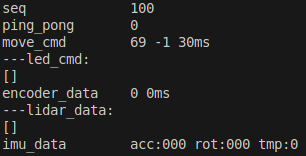
\includegraphics[width=0.5\textwidth, center]{img/Backend/print_wrapper_all.png}
    \caption{Python - Protobuf Konsolen Ausgabe}
    \label{fig:py_konsole_o}
\end{figure}

In Zukunft kann dies durch die Datenbank oder ein CSV log abgelöst werden 
und somit auch bessere Systeme implementiert werden.
% 
Diese könnten automatisch für sonderbare Änderungen suchen 
und entsprechen Melden und in einem Log abspeichern.

\subsection{Optimierungsmöglichkeiten}
\initials{JS}
\label{subsec:Optimierungsmöglichkeiten}
\subsubsection{uvloop - schnellere Koroutinen}
\initials{JS}
% uvloop - drop in replacement
% https://github.com/MagicStack/uvloop
uvloop ist ein schneller drop-in Ersetzung von der eingebauten asyncio Event Loop, 
dieser ist entsprechend in Cython entwickelt 
(Cython ist entsprechend Python aber als Performanten C code compiliert).
Ziel dieser Ersetzung ist es asyncio um einiges schneller zu machen 
aber nicht von der Referenz verhalten von asyncio abzuweichen. 
Als drop-in Ersetzung geht dies so weit, 
dass die Abweichungen als Fehler kategorisiert werden.
% 
Während der Prototyp Phase dieses Projekts 
ist man auf der Standard Implementierung geblieben, aufgrund Stabilität
und weil uvloop bis später im Projekt unbekannt geblieben ist.
In Zukunft wird jedoch eine Implementierung in Betracht gezogen,
aufgrund der vorhin genannten Eigenschaften.
% 
Insbesondere wenn die nachfolgenden Projekte weiter skalieren.

% compelierung python code
\subsubsection{Kompilierung}
\initials{JS}
Es ist möglich Python code genau so wie jedes andere Programm zu kompilieren,
jedoch ist dies standardmäßig nicht nötig 
da der Interpreter Cpython automatisch Python byte code kompeliert (in PYC Dateien).
Das prekompilieren wird hauptsächlich dafür verwendet um die Start zeit zu verringern 
und um den Code für die gewählte Platform einfacher zu verteilen,
weil man keine weiteren Pakete installieren muss sondern
nur die PYC Datei allein genügt.
% Dies ist jedoch für dieses Projekt irrelevant.

\subsection{threading vs asyncio}
\initials{JS}
% TODO threading warum nicht streng nötig 
% (hauptsächlich limitiert über Wifi I/O nicht anzahl an geräten & )
% falls anzahl größer wird dann villeicht

\section{Probleme}
\initials{JS}
\subsection{Linux Modifikationen}
\initials{JS}
Es kam das Problem auf, dass die lokale IP suche auf Linux Ubuntu nicht funktionierte.
Dies lag daran, dass die vorherige Variante, 
welcher mithilfe der Domain Name auf die lokale IP-Adresse findig wurde.
Jedoch wurde auf Linux eine andere Adresse zurückgeliefert, 
zwar die Loopback-Adresse \texttt{127.0.1.1}. 
Diese Adresse wird verwendet, um den \texttt{host\_name} eine Adresse zuzuweisen,
im Falle das kein Netzwerk vorhanden ist. 
Sonst kann eine permanente IP-Adresse hier zugewiesen werden.
% https://askubuntu.com/questions/754213
% /what-is-difference-between-localhost-address-127-0-0-1-and-127-0-1-1

Als Lösung öffnet das Programm temporär ein Socket 
und findet mit dieser die lokale IP-Adresse, und dadurch Plattform unabhängig.
\begin{lstlisting}[language=python, gobble=4]
    import socket

    def get_local_ip():
    """
    opens a temporary socket connection and retrieves the local IP
    """
    s = socket.socket(socket.AF_INET, socket.SOCK_DGRAM)
    try:
        # doesn't even have to be reachable
        s.connect(('10.255.255.255', 1))
        IP = str(s.getsockname()[0])
    except Exception as b:
        print("error at figuring out local ip")
        print(b)
        exit
    finally:
        s.close()
    return IP
\end{lstlisting}

\subsection{Potenzielles blockierendes verhalten}
\initials{JS}
% bot_handler und server nicht separat gestartet werden.
Obwohl die Kommunikation in hauptsächlich zwei  teile aufgeteilt ist, mit 
Bot Händler und Server, 
jedoch werden sie zu diesem Zeitpunkt gesammelt und gemeinsam gestartet.
Dies führt zu einer womöglich ungewollten Konsequenz,
dass falls der Bot Händler sich frühzeitig oder ungewollt beendet, 
nicht neu gestartet wird bis sich einen neuen Client verbindet.
% 
Da jedoch für diese Diplomarbeit zu erwarten ist, 
dass die Bots stets zur Verfügung stehen sollten,
wird der Prozess, bei einer geschlossenen Verbindung,
für eine gewisse Zeit pausiert bevor ein neuer Verbindungsversuch gestartet wird.

In den nächsten Iterationen sollten jedoch 
die zwei Aufträge unabhängig gestartet werden können, 
um die Situation zu vermeiden, dass die ganze Kommunikation neu gestartet werden muss.

\subsection{Protobuf Generierung}
\initials{JS}
% siehe server/README.md
% verlege zu Backend probleme?
Während des migrieren vom Vorentwicklungs Ordner, 
aufgrund dessen das es noch nicht klar wie mit Protobuf 
und der neuen Websocket Implementation zu hantieren ist, 
wurde für eine gewisse Zeit in einem Testordner experimentiert.
Dies führte dazu das der generierte Protobuf code nicht funktionierte,
da der Wrapper nicht über den Unterordner Standort \text{protobuf/}, 
der weiteren Protobuf-dateien informiert wurde.
Da die compilieren der Protobuf Dateien für Python unabhängig vom Standort
der Python Umgebung geschieht. 
Wodurch die Importe im generierten \text{wrapper\_pb2.py}
mit dem Ordner prefixed werden müssen.

\begin{lstlisting}[language=python, gobble=4]
    import protobuf.move_cmd_pb2 as move__cmd__pb2
    import protobuf.led_cmd_pb2 as led__cmd__pb2
    import protobuf.lidar_data_pb2 as lidar__data__pb2
    import protobuf.encoder_data_pb2 as encoder__data__pb2
    import protobuf.imu_data_pb2 as imu__data__pb2
\end{lstlisting}


% \section{Protobuf Generierung}
% \initials{JS}
% TODO schreib ein skript dafür

% \section{Konfiguration Datei}
% \initials{JS}
% TODO schreib ein skript dafür

\section{Test Codes}
\initials{JS}
Es wurden weitere allgemeinere Test Codes geschrieben, 
welche die Funktion dienten, die Kommunikation Kanäle und Daten Bearbeitung innerhalb 
und außerhalb des Backends zu testen und gegebenenfalls 
von anderen Team Mitglieder modifiziert.
% 
Aber auch für die Fehlersuche 
und sind im Allgemeinen eine Schnelle Option 
um die Kommunikation und Datentausch zu testen.

Diese Codes haben große Ähnlichkeiten mit der Prototyp Kommunikation, 
deshalb wird in diesem Abschnitt hauptsächlich auf deren Nutzen eingegangen.

\subsection{Einzelverbindung - Robot\_ws\_test.py}
\initials{JS}
Dieser Testcode ist verantwortlich sich mit den Bots zu verbinden 
und dessen Daten zu lesen.
Es wurde mit einigen Konfigurationen erweitert und modifiziert, 
und wird im Laufe des Projektes angepasst, wenn nötig.
Zurzeit wurde es bereits verwendet, um die Kommunikation zu testen, 
die Bearbeitung von erhaltenen Daten vom Bot und genereller Fehler suche.

\subsection{Client und Server}
\initials{JS}
Dazu gehören \texttt{test\_wrap\_client.py} (als den Frontend) 
und \texttt{test\_wrap\_bot\_transceiver.py} (als die Bots).
Diese sind einfache Codes welcher Client uns Server (Bots und Server) emuliert, 
indem sich beide Protobuf Pakete zueinander schicken. 
Diese sind dienen hauptsächlich zum Testen der Websocket Kommunikation 
und auch zur Übung wie Protobuf in Python zu verwenden sind, 
und nehmen die Position des Frontends und Bots.
Die zwei Senden und Empfangen die Protobuf Wrapper über die Backend Kommunikation 
und geben diese in die Konsole aus.
